% Author -- bikz05
\documentclass[11pt]{article}
%Gummi|065|=)
\date{}

% Geometry
\usepackage[margin=1in]{geometry}
\usepackage{graphicx}
% Start paragraph from new line
\usepackage{parskip}
% Links
\usepackage{hyperref}
\usepackage{url}
% Prevent figures from going on next page
\usepackage{float}
% Quotes
% Color
\usepackage{color}
% Codes
\usepackage{verbatim}
%\usepackage{listings}
% For subcaptions     
\usepackage{subcaption}
% For Algorithms
\usepackage{pkgs/algorithm2e}
% For Source Code
\usepackage{amsmath}
\usepackage{bm}
% For Bib
% TODO
%\usepackage{cite}
\usepackage[numbers]{natbib}
\usepackage{notoccite}
% To add gifs
\usepackage{movie15}

\begin{document}


\begin{titlepage}

\newcommand{\HRule}{\rule{\linewidth}{0.5mm}} % Defines a new command for the horizontal lines, change thickness here

\center % Center everything on the page
 
%----------------------------------------------------------------------------------------
%	HEADING SECTIONS
%----------------------------------------------------------------------------------------

\textsc{\LARGE University Name}\\[1.5cm] % Name of your university/college
\textsc{\Large Major Heading}\\[0.5cm] % Major heading such as course name
\textsc{\large Minor Heading}\\[0.5cm] % Minor heading such as course title

%----------------------------------------------------------------------------------------
%	TITLE SECTION
%----------------------------------------------------------------------------------------

\HRule \\[0.4cm]

{ \huge \bfseries Title of Document}\\[0.4cm] % Title of your document

%\includegraphics[scale=.4]{figures/simplegrasping.jpg}

\HRule \\[1.5cm]
 
%----------------------------------------------------------------------------------------
%	AUTHOR SECTION
%----------------------------------------------------------------------------------------

\begin{minipage}{0.4\textwidth}
\begin{flushleft} \large
\emph{Author:}\\
Bikramjot \textsc{Hanzra} \\

\end{flushleft}
\end{minipage}
~
\begin{minipage}{0.4\textwidth}
\begin{flushright} \large
\emph{Instructor:} \\
Supervisor's Name % Supervisor's Name
\end{flushright}
\end{minipage}\\[2cm]

% If you don't want a supervisor, uncomment the two lines below and remove the section above
%\Large \emph{Author:}\\
%John \textsc{Smith}\\[3cm] % Your name

%----------------------------------------------------------------------------------------
%	DATE SECTION
%----------------------------------------------------------------------------------------

{\large February 12, 2016}\\[2cm] % Date, change the \today to a set date if you want to be precise

%----------------------------------------------------------------------------------------
%	LOGO SECTION
%----------------------------------------------------------------------------------------

%
\includegraphics[scale=.2]{figures/logo.eps}\\[1cm] % Include a department/university logo - this will require the graphicx package
 
%----------------------------------------------------------------------------------------

\vfill % Fill the rest of the page with whitespace

\end{titlepage}


\tableofcontents
%\lstinputlisting[language=Octave]{BitXorMatrix.m}

\listoffigures

\pagebreak

\section{Introduction}

Below is how to write algorithms -- \\
\begin{algorithm}[H]
\SetAlgoLined
\KwResult{Execute grasp}
 \While{not SUCCESS}{
 \begin{enumerate}
 \item  Select Preshape -- \emph{High-dimensional hand posture space}\\
\item Select Pose -- \emph{Diversity (Clutter, Arm reachability)} \\
\item Select Controller -- \emph{Realism} \\
\item Run Controller -- \emph{Computation Time} \\
\item Verification -- \emph{Post-grasp stability, Uncertainty}
 \end{enumerate}
 }
 \caption{Process in Simulation with issues involved}
 \label{algo}
\end{algorithm}

Matrices can be written as below --

$$C_H = \begin{bmatrix}
	\theta_1 \\ 
	\theta_2 \\
\end{bmatrix}$$

Code can be added as --

\begin{verbatim}
$$C_H = \begin{bmatrix}
	\theta_1 \\ 
	\theta_2 \\
\end{bmatrix}$$
\end{verbatim}

Also, Inline code can be added as using \texttt{\textbackslash texttt\{text\}}.

\pagebreak

Figures can be added as --

\begin{figure}[H]
	\centering
	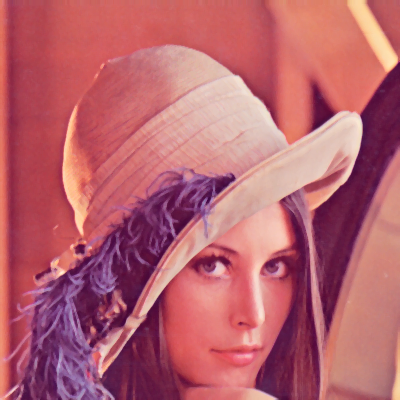
\includegraphics[scale=1]{figures/lena.png}
    \caption{Caption 1}
    \label{label1}
\end{figure}%

Sub-figures can be added as --

\begin{figure}[H]
    \centering
    \begin{subfigure}[t]{0.5\textwidth}
        \centering
		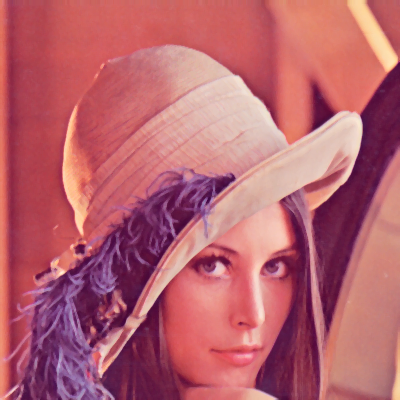
\includegraphics[scale=.4]{figures/lena.png}
        \caption{\emph{Caption 1 }}
    \end{subfigure}%
    ~
    \begin{subfigure}[t]{0.5\textwidth}
        \centering
        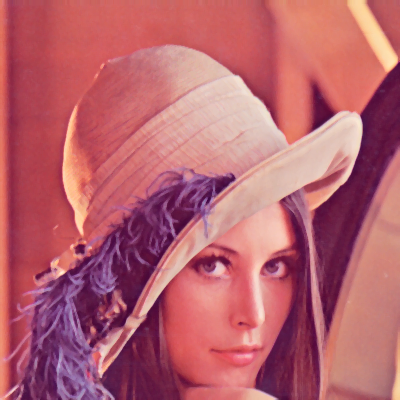
\includegraphics[scale=.4]{figures/lena.png}
		\caption{\emph{Caption 2}}
    \end{subfigure}%

    \begin{subfigure}[t]{0.5\textwidth}
        \centering
		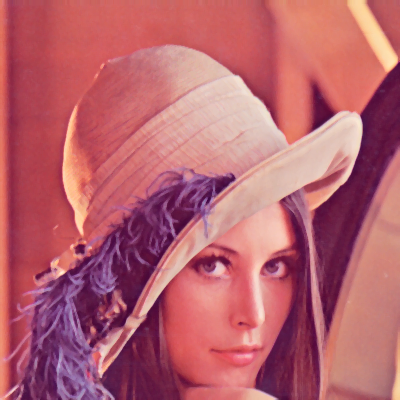
\includegraphics[scale=.4]{figures/lena.png}
        \caption{\emph{Caption 3}}
    \end{subfigure}%
    ~
    \begin{subfigure}[t]{0.5\textwidth}
        \centering
        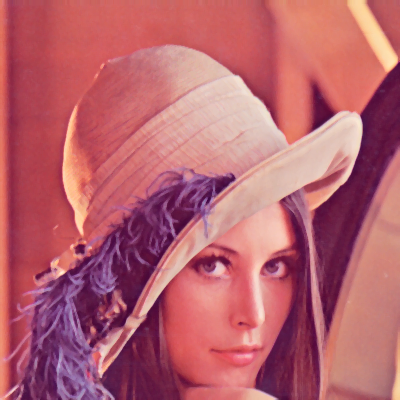
\includegraphics[scale=.4]{figures/lena.png}
		\caption{\emph{Caption 4}}
    \end{subfigure}%
    \caption{Caption 2}   
    \label{Label 2} 
\end{figure}

\bibliographystyle{unsrtnat}
\bibliography{grasping-scribes}

\hrulefill 

\end{document}
